\section{安装Flume}
\subsection{简介}
在电商、销售等各类系统中,日志是一种非常重要的信息载体,应用会产生大量的日志信息。
将不同形式、不同渠道的日志收集起来非常重要且困难。
Flume是一种可靠的分布式日志收集工具。能够通过定义源Sources、通道Channels和目的地Sinks,方便各种日志信息的收集,汇总到HDFS中,方便后续
的通过Mapreduce或者Hive、HBase等的分析处理。

\subsection{安装配置}

Flume的安装和配置非常的容易,主要是\lstinline{flume-env.sh}和\lstinline{flume.conf}
两个文件。

\lstinputlisting[style=mysh, title=flume-env.sh]{docs/flume/conf/flume-env.sh}

在\lstinline{flume-env.sh}中写入\lstinline{JAVA_HOME}的位置即可。

Flume的运行需要通过\lstinline{flume.conf}来指定,下面是\lstinline{flume.conf}的一个配置实例。

\lstinputlisting[style=mysh, title=flume-conf.properties]{docs/flume/conf/flume-conf.properties}

在Flume的配置文件中,需要指定一个Agent。Agent内部包含了Sources、Channels和Sinks。
表明了日志数据的流动方向。下面是Flume的架构图:

\begin{figure}[h]
	\centering
	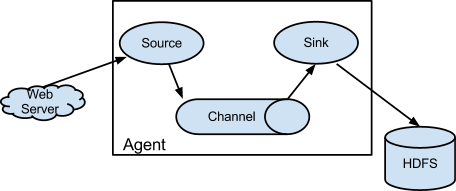
\includegraphics[width=0.6\linewidth]{flume/flume_arch.png}
	\caption{Flume的基础架构}
	\label{fig:flume_arch}
\end{figure}

在上面这个例子中,指定了Agent的名称为\lstinline{agent},Agent的日志来源是\lstinline{seqGenSrc},
Agent的通道是\lstinline{memoryChannel}内存,Agent的目的地是\lstinline{loggerSink}。

注意这里指定的都是名称,在后面\lstinline{.type}具体指定类型。

在指定完类型后,\lstinline{agent.sources.seqGenSrc.channels}和\lstinline{agent.sinks.loggerSink.channel}分别
指定了源的通道和目的地的通道,这就像是将源端与目的端连接起来了一样。这里要注意\lstinline{channels}和\lstinline{channel}
的区别,在Flume中,一个源是可以和多个Channel对应的,而一个目的与一个Channel对应。可以在拓扑逻辑上
见到它们的区别,这里的配置也表明了这一点。

运行这个例子需要输入以下命令:

\lstinputlisting[style=mysh,title=启动Flume自动的配置模板]{docs/flume/use-conf-temp.sh}

其中,\lstinline{-c}指明配置文件的目录,在有多个配置文件和需要找到\lstinline{JAVA_HOME}时都需要。\lstinline{-f}指定读取那个配置文件,\lstinline{-n}表示Agent的名称。

\subsection{测试和运用}

如上节所介绍,Flume的运行主要通过指定配置来指定。
Flume的日志来源、通道和目的地都可以很多,灵活搭配使用。下面是一个Example,

\lstinputlisting[style=mysh,title=example.conf]{docs/flume/conf/example.conf}

上面的配置定义了一个名称为\lstinline{a1}的Agent,监听44444端口上的数据作为
输入的源、一个在内存中的缓冲作为事件的通道,并且将控制台日志输出作为事件的目的地。
通过下面命令启动:

\lstinputlisting[style=mysh,title=启动监听端口的例子]{docs/flume/start-example.sh}

在启动后,新建一个窗口,或者将终端分屏,使用\lstinline{telnet}向44444
端口发送数据,可以检测到Flume监听端接收到数据。

\begin{figure}[h]
	\centering
	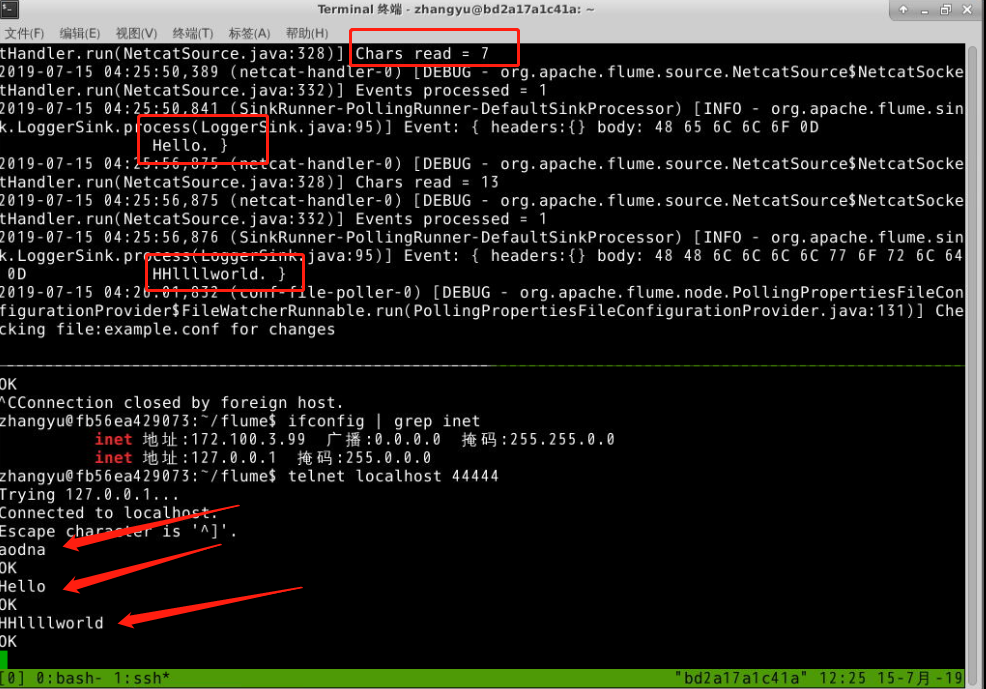
\includegraphics[width=\linewidth]{flume/flume-example.png}
	\caption{监听Telnet的例子}
	\label{fig:flume_example}
\end{figure}
